\documentclass{salt}
\usepackage{linguex}
% This document template was developed by the editors of /Semantics and
% Pragmatics/ and minimally modified to work with the salt.cls document class.

\usepackage[equation]{gb4e-salt}
\noautomath
\newcommand{\sem}[2]{\mbox{$\llbracket${#2}$\rrbracket^{#1}$}} 
\newcommand{\seq}[1]{\left\langle {#1} \right\rangle}
\newcommand{\ul}{$\ulcorner$}
\newcommand{\ur}{$\urcorner\ $}
\newcommand{\urn}{$\urcorner$}
\newcommand{\reff}[1]{(\ref{#1})}
%=====================================================================
%========================= preamble material =========================

% Metadata for the PDF output. ASCII-only!
\pdfauthor{Matthew Mandelkern and Jonathan Phillips}
\pdftitle{Sticky situations: `Force' and quantifier domains}
\pdfkeywords{Moral psychology; `force'; quantifier domains; experimental semantics and pragmatics; Knobe effect}

% Short title inside square brackets, for the running headers.
% If no short title is given, no title appears in the headers.
% Please use sentence case for the title.
\title[Sticky situations: \emph{Force} and quantifier domains]{Sticky situations: \emph{Force} and quantifier domains\thanks{Thanks to several anonymous referees and the audience at \emph{SALT} 28; audiences at the University of Chicago and \emph{SPP} 2017; and to Michael Glanzberg, Angelika Kratzer, and Ginger Schultheis, for very helpful comments and discussion.}}



% Optional short author inside square brackets, for the running headers.
% If no short author is given, no authors print in the headers.
\author[Mandelkern and Phillips]{%
  % As many authors as you like, each separated by \AND.
  \saltauthor{Matthew Mandelkern \\ \institute{All Souls College, Oxford}} \AND
  \saltauthor{Jonathan Phillips \\ \institute{Harvard University}}%
}
%=====================================================================
\frenchspacing
\begin{document}

%=====================================================================
%============================ frontmatter ============================

\maketitle

% First page headers and page numbers; update these when you are assigned final
% page numbers
%
% the page number of the first page of this paper
\setcounter{page}{1}

% Create the first page headings.
% This needs to be issued *after* \maketitle.
% \firstpageheadings{<volume>}{<first page>}{<last page>}{<year>}{}{}
\firstpageheadings{28}{000}{000}{2018}{}{}

\begin{abstract}  
When do we judge that someone was forced to do what they did? One relatively well-established finding is that subjects tend to judge that agents were not forced to do actions when those actions violate norms. A surprising discovery of \citealt{young2011paradox} is that this effect seems to disappear when we frame the relevant `force'-claim in the active rather than passive voice (\ul $X$ forced $Y$ to $\varphi$\ur vs. \ul$Y$ was forced to $\varphi$ by $X$\urn). Young and Phillips found a similar contrast when the scenario itself shifts attention from $Y$ (the forcee) to $X$ (the forcer). We propose that these effects can be (at least partly) explained by way of the role of attention in the setting of quantifier domains which in turn play a role in the evaluation of `force'-claims. We argue for this hypothesis by way of an experiment which shows that sequences of active vs. passive `force'-claims display the characteristic ``stickiness'' of quantifier domain expansion, using a paradigm which we argue provides a useful general paradigm for testing quantifier domain hypotheses. Finally, we sketch a semantics for `force' which we argue is suitable for capturing these effects. 
\end{abstract}

\begin{keywords}
 moral psychology, `force', quantifier domains, experimental semantics and pragmatics, Knobe effect
\end{keywords}



\section{Introduction}

A wide variety of studies in recent years have shown that judgments about morality have surprising ramifications in apparently distinct conceptual domains, in particular having to do with causality and intentionality. Among other things, judgments about morality influence judgments about whether someone was forced to do what they did. In this paper we aim to improve our understanding of this phenomenon by making a case study of subtle variations in these judgments identified by \citet{young2011paradox}. We argue that these judgments are best explained by way of a hypothesis which connects judgments about `force' to quantification over a domain which we call a \emph{causal background}: a set of propositions which represent the causal structure of a particular situation. The more causes we take into account, the more likely we are to judge that someone was forced to do what they did.

%We begin by reviewing the basic phenomenon: subjects are less likely to agree that an individual was forced to do $\varphi$ if $\varphi$ is judged to be a morally bad action than if it is morally neutral. A more recent, and surprising, discovery of \citealt{young2011paradox} is that this effect seems to disappear when we focus on the active rather than passive version of the sentences in question. We replicate this effect using `As far' clauses which focus attention on either the forcer or the forcee. Based on this, we propose that both affects should be explained by way of the function of \emph{attention} in assessing `force'-claims. In particular, we propose that attention can affect the setting of a quantifier domain which represents the causal background of the scenario in question. We test for this hypothesis by way of an experiment which tests judgments about \emph{sequences} of `force'-claims with different attention conditions; the results of this experiment, we argue, clearly show the characteristic pattern of quantifier domain expansion. [[We say SOMETHING, WHAT, finally, about how to encode the basic Knobe effect. ]]

%We close by emphasizing two methodological upshots: first, we take our proposal to show that  work in formal semantics and pragmatics can help with moral psychology, and \emph{vice versa}; second, we argue that our sequence experiment provides a widely applicable experimental operationalization of hypotheses that the interpretation of something goes by way of a quantifier domain. 

%We explain these order effects as follows. Judgments about \emph{force} vary with a contextually given parameter, which is sensitive to how much information about the causal background we are taking into account. The more causal background we take into account, the less we are inclined to judge that someone could have done otherwise than they in fact did, and thus the more we are willing to judge that they were forced to do what they did. We hypothesize that when we are thinking about morality---and more generally, about matters in the broadly practical realm---we tend to ignore substantial parts of the causal background, instead conceptualizing agents as in some sense free to act in a variety of ways. But when elements of the causal background are made salient---as in the topicalization paradigm we discuss here---we can no longer ignore them, and thus tend to judge agents as less free to do otherwise---and therefore more likely to have been forced to do what they in fact did. We spell out this account by giving a semantics for \emph{force} which predicts this kind of contextual variability, but we argue that this account of the role of morality in judgments of this kind extends quite broadly to the array of concepts which make up the core of our practical lives.

\section{The basic effect}

Moral judgments influence intuitions about ostensibly non-moral issues in surprising, and now well-documented, ways (this is sometimes called the \emph{Knobe effect} after \citealt{knobe2003intentional}; see \citeyear{knobe2010person} for a review). While the basic intuition behind these phenomena can be see at least as early as Aristotle (\textit{NE} 1110$^a$8-9), an explosion of recent empirical work has shown that people's moral judgments influence their ordinary assessments of whether or not an agent acted intentionally \citep{knobe2003intentional,leslie2006acting,cova2015intentional}, whether an agent caused a given outcome \citep{alicke1992culpable,knobe2008causal, hitchcock2009cause}, whether or not an agent acted freely \citep{phillips2009moral}, and so on \citep{pettit2009pervasive,phillips2015unifying}.

Our focus here will be on the impact that moral judgments have on assessments of whether or not an agent was forced to do a given action. The first empirical work on this topic, \citealt{phillips2009moral}, randomly assigned half of participants to read each of the two variants in the following vignette; the first variant involves a morally neutral action (throwing cargo overboard) while the second involves a morally bad action (throwing a person overboard).

\begin{exe}
\ex \label{cargo} \textbf{[Cargo/Wife]} While sailing on the sea, a large storm came upon a captain and his ship.  As the waves began to grow larger, the captain realized that his small vessel was too heavy and the ship would flood if he didn't make it lighter.  The only way that the captain could keep the ship from capsizing was to throw his [wife's expensive cargo/wife] overboard.\\ \hspace*{.5cm} Thinking quickly, the captain took [her cargo/his wife] and tossed [it/her] into the sea.  While the [expensive cargo/captain's wife] sank to the bottom of the sea, the captain was able to survive the storm and returned home safely\end{exe}

\noindent After reading the vignette, participants in the cargo condition were asked whether they agreed or disagree with \reff{permissibleS}.

\begin{exe}
\ex \label{permissibleS} \textit{Cargo:} The captain was forced to throw his wife's cargo overboard.\end{exe}

\noindent Participants in the wife condition were likewise asked whether they agreed or disagree with \reff{impermissibleS}.

\begin{exe}\ex \label{impermissibleS} \textit{Wife:} The captain was forced to throw his wife overboard.\end{exe}

Participants' judgments about whether the ship captain was forced diverged in the two cases. In the morally permissible (cargo) condition, participants judged much more that the captain was forced (to throw the cargo overboard) than in the morally impermissible (wife) condition, where participants were much less inclined to judge that the ship captain was forced (to throw the passengers overboard). This phenomenon, in which people's assessments of whether someone was forced are impacted by their moral judgments about the action in question, has  been replicated and extended in a number of different ways (see \citealt{young2011paradox,chakroff2015harmful,phillips2015unifying}).

A promising recent  attempt to account for the influence of normative considerations in participants' assessments of `force' (and more generally), which we will build on in what follows, is due to \citealt{knobe2013modals}, who argue that we can capture the meaning of the sentences assessed by participants in these studies by way of a modal proxy. Thus \reff{permissibleS} could be understood as contextually equivalent to \reff{permissibleM}, and \reff{impermissibleS} could be understood as contextually equivalent to \reff{impermissibleM}.

\begin{exe}\ex \label{permissibleM} %\textit{Modal Permissible} $\approx$ 
Given the circumstances, the captain had to throw the cargo overboard.\end{exe}

\begin{exe}\ex \label{impermissibleM} %\textit{Modal Impermissible} $\approx$ 
Given the circumstances, the captain had to throw his wife overboard.\end{exe}

\noindent Knobe and Szab\'o provide evidence for this claim by replicating the earlier pattern of results using these proxy sentences. That is, they showed that participants agreed with \reff{permissibleM} but not with \reff{impermissibleM}, similar to the way in which they agreed with \reff{permissibleS} but not \reff{impermissibleS}. Knobe and Szab{\'o} then propose an account of the difference in participants' judgments by way of a semantics of modal auxiliaries, drawing largely on \citealt{Kratzer1977,Kratzer:1981}, but argue that the domain of possibilities quantified over by  modal auxiliaries in these cases is of an ``impure'' flavor, meaning that deontic considerations partially determine which possibilities are included in the domain. In particular, they appeal to a principle they call \emph{Hope}, which ensures that the relevant modal domain always contains a possibility in which no contextually salient norms are violated. As they point out, \reff{impermissibleM} will be false as long as there is some possibility in the domain in which the contextually salient norm against murder is not violated. By contrast, this principle will not affect the truth value of \reff{permissibleM}, since throwing cargo overboard does not violate a salient norm. Thus, assuming \reff{impermissibleS} is contextually equivalent to \reff{impermissibleM} and \reff{permissibleS} is contextually equivalent to \reff{permissibleM},  Knobe and Szab\'o  are able to derive the difference in force judgments.

\section{Attention affects} \label{sec:part1}

We think that Knobe and Szab\'o's idea is promising, and we will build on the basic idea here, trying to refine it in what follows by giving a more explicit semantics for `force' and providing independent evidence that judgments in these cases are indeed sensitive to quantifier domains. The starting point for our discussion is the striking discovery from \citealt{young2011paradox} that the effect summarized in the last section is sensitive to whether subjects are presented with an active or a passive variant of the `force' ascription. For example, Young and Phillips asked participants to read either the cargo or passenger variant of \reff{youngScenario}:

\begin{exe}\ex While sailing on the sea, a large storm came upon a captain and his ship. As the waves began to grow larger, the captain realized that his small vessel was too heavy and the ship would flood if he didn't make it lighter. The only way that the captain could keep the ship from capsizing was to throw his [expensive cargo/passengers] overboard. Thinking quickly, the captain ordered one of his sailors to throw the [cargo/passengers] overboard. While the [cargo/passengers] sank to the bottom of the sea, the captain was able to survive the storm and returned home safely. \label{youngScenario}\end{exe}


\noindent In this scenario, Young and Phillips replicated the basic effect of morality with questions like \reff{12}:

\begin{exe}\ex \label{12} Was the sailor forced to throw the [cargo/passengers] overboard?\end{exe}

\noindent That is, as expected, Young and Phillips found that subjects were more inclined to answer affirmatively to \reff{12} in the cargo condition than in the passenger condition, just as one would expect given the findings summarized above. Surprisingly, however, Young and Phillips found no similar effect when they asked participants about \reff{13}: 

\begin{exe}\ex \label{13} Did the captain force the sailor to throw the [cargo/passengers] overboard?\end{exe}

\noindent Rates of affirmative answers to \reff{13} did not vary significantly across the two conditions (passengers vs. cargo). This is surprising, because \reff{13} is just the active form of the passive question in \reff{12}, and, on the face of it, is intuitively equivalent to it. 

It is not immediately clear how Knobe and Szab{\'o}'s proposal can on its own account for this kind of difference. Their \emph{Hope} principle is meant to be quite general, and thus one would think participants would be just as unwilling to agree that the captain forced the sailor to throw the passengers overboard as they are to agree that the sailor was forced to throw the passengers overboard by the captain; in both cases, one would expect \emph{Hope} to require that the domain include possibilities in which the sailor does not violate the contextually salient norm against murder, and thus one would not expect participants to agree that the captain forced the sailor to throw the passengers overboard any more than they agree that the sailor was forced to throw the passengers overboard. 

What then might explain this pattern? One possibility we find promising, following Young and Phillips' own interpretation of the data, is that the explanation does not have to do with the particular semantics of the passive, but rather with the fact that \reff{13} draws attention to the captain more than \reff{12} does. Support for this kind of explanation of this difference comes from another study reported by Young and Phillips \citeyearpar{young2011paradox}, in which they varied whether the vignette itself focused participants' attention on the role of the captain or on the role of the sailor, as in the two versions of \reff{focus}.

\begin{exe}\ex While he was sailing on the sea, a large storm came upon a [sailor/captain] on a ship. The waves began to grow larger, and the [sailor's/captain's] small vessel was too heavy. The [sailor's/captain's] ship would flood and the [sailor/captain] would drown if he didn't make it lighter. The only way that the [sailor/captain] could keep the ship from capsizing was to throw the passengers overboard. Thinking	quickly, the captain of the ship ordered the sailor to throw the passengers overboard. The sailor threw the passengers overboard. While the passengers sank to the bottom of the sea, the [sailor/captain] was able to survive the storm and returned home safely.
\label{focus}\end{exe}

\noindent Participants were observed to agree significantly more with \reff{13} when their attention had specifically been drawn to the role of the captain rather than the sailor. These findings fit naturally with an approach to Young and Phillips' data on which the key factor affecting the contrast between the active and passive variations has to do with the change in attention these two constructions naturally bring out between the forcer and the forcee, respectively. In more detail, we will suggest that drawing attention  to the captain's causal role in bringing it about that the sailor threw the [cargo/passengers] overboard makes it more likely that participants take the captain's causal influence into account in assessing whether the sailor was forced to act as he did. 



\section{Domain expansion}\label{sec:part2}

Why does calling attention to the \emph{forcer} lead to increased agreement with `force' sentences in the immoral (passenger) condition, while calling attention to the \emph{forcee} leads to decreased agreement in that condition? This is the question that we will focus on in the rest of this paper. Our hypothesis is that attentional variation affects the setting of a {quantifier domain} which plays a part in the interpretation of `force'. 

This is a \emph{prima facie} natural hypothesis given that, in general, drawing attention to things---objects, possibilities, actions---can change judgments about the truth-value of sentences that involve quantificational structures. This hypothesis is also in line with the general strategy pursued by Knobe and Szab\'o above, on which modal quantifier domains play a crucial role in explaining the observed judgments. Importantly, if this claim is right, then it will help resolve the paradox that Young and Phillips identify regarding the effect of attention on `force' judgments, i.e., that participants agree with `The captain forced the sailor to throw the passenger overboard' while disagreeing with `The sailor was forced to throw the passenger overboard by the captain'. While this combination of attitudes appears inconsistent at first, if the meaning of these sentences varies with the domain made salient by context, then it may turn out that there is nothing truly inconsistent about this combination of judgments.

Let us begin by considering a few examples that illustrate in a general way the role of attention in quantifier domain expansion. One place that this kind of effect can be seen is in the domain of generalized quantifiers like `all', `some', `no', and so on. Suppose Ted has just finished the last beer in his house; then \reff{beer1} sounds reasonable.

\begin{exe}\ex There's no more beer.\label{beer1} \end{exe}

\noindent Here Ted is only talking about the beer in his house: the domain of his quantifier ranges only over the things in the house. But now suppose Mark responds with \reff{respm}: 

\begin{exe}\ex Sure there is---at the liquor store!\label{respm}\end{exe}

\noindent With his response, Mark is calling attention to beer that Ted was (quite reasonably) neglecting. This response seems to \emph{expand} the salient domain of quantification for `no'. An important feature of cases like this, observed by \citet{LewisScorekeeping}, is that once our attention has been called to the beer in the liquor store, it is no longer easy to ignore that beer. Ted can complain that Mark's response is pedantic, unhelpful, and obnoxious; but it seems difficult, after Mark's response, for Ted to stand his ground and insist that \reff{beer1} is true.
 
 Importantly for present purposes, we find similar effects in broadly modal domains. For instance, in the case of knowledge ascriptions---which, following \citealt{Hintikka62}, we can treat as universal quantifiers over a set of possible worlds---simply drawing attention to skeptical possibilities makes it harder to subsequently ignore them (and  thus harder to subsequently ascribe knowledge; see \citealt{DeRose1991,Lewis1996}). Likewise, in the case of conditionals---which, following \citealt{Stalnaker68, Lewis:1973,Kratzer:1981} are standardly treated as devices for talking about worlds in a given domain of accessible worlds---calling attention to certain outlying possibilities makes it harder to subsequently ignore them. A pair of sequences, from \citealt{Lewis:1973} (attributed to J.\ Howard Sobel) and \citealt{vonFintelCIDE} (attributed to Irene Heim), illustrates this phenomenon nicely: 
 
 \begin{exe}\ex\begin{xlist} \label{rf1}\ex\label{10} If the USA threw its weapons into the sea tomorrow, there would be war. \ex \label{11} But if the USA and the other nuclear powers all threw their weapons into the sea tomorrow, there would be peace.\end{xlist}\end{exe}
 
  \begin{exe}\ex\begin{xlist}\ex  If the USA and the other nuclear powers all threw their weapons into the sea tomorrow, there would be peace. \ex ?? But if the USA threw its weapons into the sea tomorrow, there would be war. \label{secondco}\end{xlist}\end{exe}
 
\noindent In the first case, both conditionals sound true. But when the order is reversed in the second case, so that the outlying possibility of all powers eliminating nuclear weapons is raised \emph{first}, it is harder to then ignore that possibility and hear a true reading of the second conditional \reff{secondco}.
  
 A final example, which comes closest to our present topic, concerns judgments about ability and freedom. \citet{Hawthorne:2001} argues that judgments about ability and freedom are sensitive to domain shifts in similar ways to knowledge ascriptions. Suppose that John eats a bagel. He says: 
 
 \begin{exe}\ex I was able to do otherwise than eat a bagel.\label{able}\end{exe}
 
\noindent  There are contexts in which we would naturally judge \reff{able} to be true. But as more and more of the causal background of John's actions is made salient, our inclination to do so somehow diminishes. As Hawthorne puts it: \begin{quote}Were I to have embarked on increasingly philosophical reflection, noting first the neurological springs of my action and then, indeed, that my act the laws of nature over which I had no control, coupled with the distribution of microparticles in the distant past over which I had no control,$\dots$I would then find myself in the position where I could no longer with good conscience ascribe to myself free will concerning whether or not I had a bagel. As I think harder about the range of determinants of my action, my inclination to ascribe freedom of choice to myself withers.\hfill \citep[p. 66-67]{Hawthorne:2001}\end{quote}

\noindent And, intuitively, this kind of domain expansion, once again, seems difficult to reverse: once we tend to the full range of an action's causal background, we are less inclined regard actions as having been done freely. 


\section{Operationalizing domain expansion}

One feature of domain expansion which we find across all these different domains is its order asymmetry. Across these different domains, it appears to be easier to {expand} domains than to shrink them; once a thing or a possibility is made salient, it is difficult to subsequently ignore it. This characteristic signature of domain expansion makes it possible to test  domain expansion hypotheses in a systematic way. At a general level, if $A$ and $A'$ mean the same thing except that $A'$ expands a quantifier domain, then, in a sequence of assertions $\seq{A, A'}$, we predict that rates of agreement with $A$ will differ from rates of agreement with $A'$. By contrast, in a sequence $\seq{A',A}$, rates of agreement will stay constant, since the first assertion introduces an expanded domain which persists for the second. This, in turn, means that we can test quantifier domain hypotheses by presenting subjects with sequences of this form, and checking whether we find the expected ``sticky'' signature of quantifier domain expansion. In this section, we use this test to explore whether the variation in judgments of passive vs. active `force' sentences can be explained by the expansion of a quantifier domain.


\subsection{Methods}

We tested our quantifier domain hypothesis about `force' by exploring ordinary judgments in sequences of `force'-claims like the following: 

\begin{exe}\ex \label{sail-capt} $\seq{passive,~ active}$: \begin{xlist}\ex The sailor was forced to throw the [passengers/cargo] overboard by the captain. \ex The captain forced the sailor to throw the [passengers/cargo] overboard. \end{xlist}\end{exe}

\begin{exe}\ex \label{capt-sail} $\seq{active,~ passive}$: \begin{xlist}\ex The captain forced the sailor to throw the [passengers/cargo] overboard. \ex The sailor was forced to throw the [passengers/cargo] overboard by the captain. \end{xlist}\end{exe}

\noindent If the variation in judgments between active and passive forms is indeed due to quantifier domain expansion, then we should find evidence for the characteristic pattern of domain expansion just surveyed: flat judgments at a fixed level $d$ in one order, and a shift in judgments in the other order, from a first judgment at a  level different from $d$, to a subsequent judgment close to $d$.

The predictions, sample size, materials, and analysis plan were all pre-registered before data were collected (\url{https://aspredicted.org/6qa2t.pdf}). All of the data, materials, and analysis code are also available (\url{https://osf.io/crxdq/}). We aimed for a sample size of 800 and recruited 812 participants in total ($M_{age}=36.65$, $SD_{age}=11.89$; 483 females, 2 unreported) from Amazon Mechanical Turk (https://www.mturk.com) \citep{buhrmester2011amazon}. Participant recruitment was automated through TurkPrime to prevent repeat participation and limit recruitment to participants with a previously established high approval rate. Participants were randomly assigned to read either the passengers or the cargo version of the following scenario: 

\begin{exe}\ex While sailing on the sea, a large storm came upon a captain and his ship. As the waves began to grow larger, the captain realized that his small vessel was too heavy and the ship would flood if he didn't make it lighter. \\ \hspace*{.5cm}The only things on the captain's small boat were a single sailor, some small but expensive cargo that he was transporting, and a number of passengers. He knew he had to throw something overboard to keep the ship from capsizing. Thinking quickly, the captain ordered the sailor to throw the [passengers/cargo] overboard. While the [passengers/cargo] sank to the bottom of the sea, the captain and his ship survived the storm and returned home safely.\end{exe}

\noindent After reading, participants were sequentially asked to indicate their agreement with two `force' statements, one passive and the other active---given either in $\seq{passive,~ active}$ order, as in \reff{sail-capt},  or in the $\seq{active,~ passive}$ order, as in \reff{capt-sail}. In all cases, participants responded on a scale from 0 (`Disagree') to 100 (`Agree'). They then completed a brief demographic form, and were thanked for their time.

\subsection{Results and discussion}

We did not exclude any participants from the analysis. Participants' agreement ratings were analyzed using the lme4 package in \textbf{\textsf{R}} \citep{bates2014lme4} by comparing a series of linear mixed-effects models, with morality (passengers vs. cargo) and sentence sequence (\reff{sail-capt} vs. \reff{capt-sail}) as between-subjects fixed factors, and judgment-order (judged first vs. judged second) as a within-subjects fixed factor. The significance of the effects was calculated by comparing a model that included the term in question to a model that differed only in excluding that term \citep{barr2013random}.

Using this approach, we observed the predicted three-way interaction between morality, sentence sequence, and judgment order $\chi^2(1)= 31.154$, $p < .001$ (Fig. \reff{Fig1}). We decomposed this by investigating the relationship between sentence sequence and judgment order when the passengers vs. cargo were thrown overboard.


\begin{figure}[ht]
	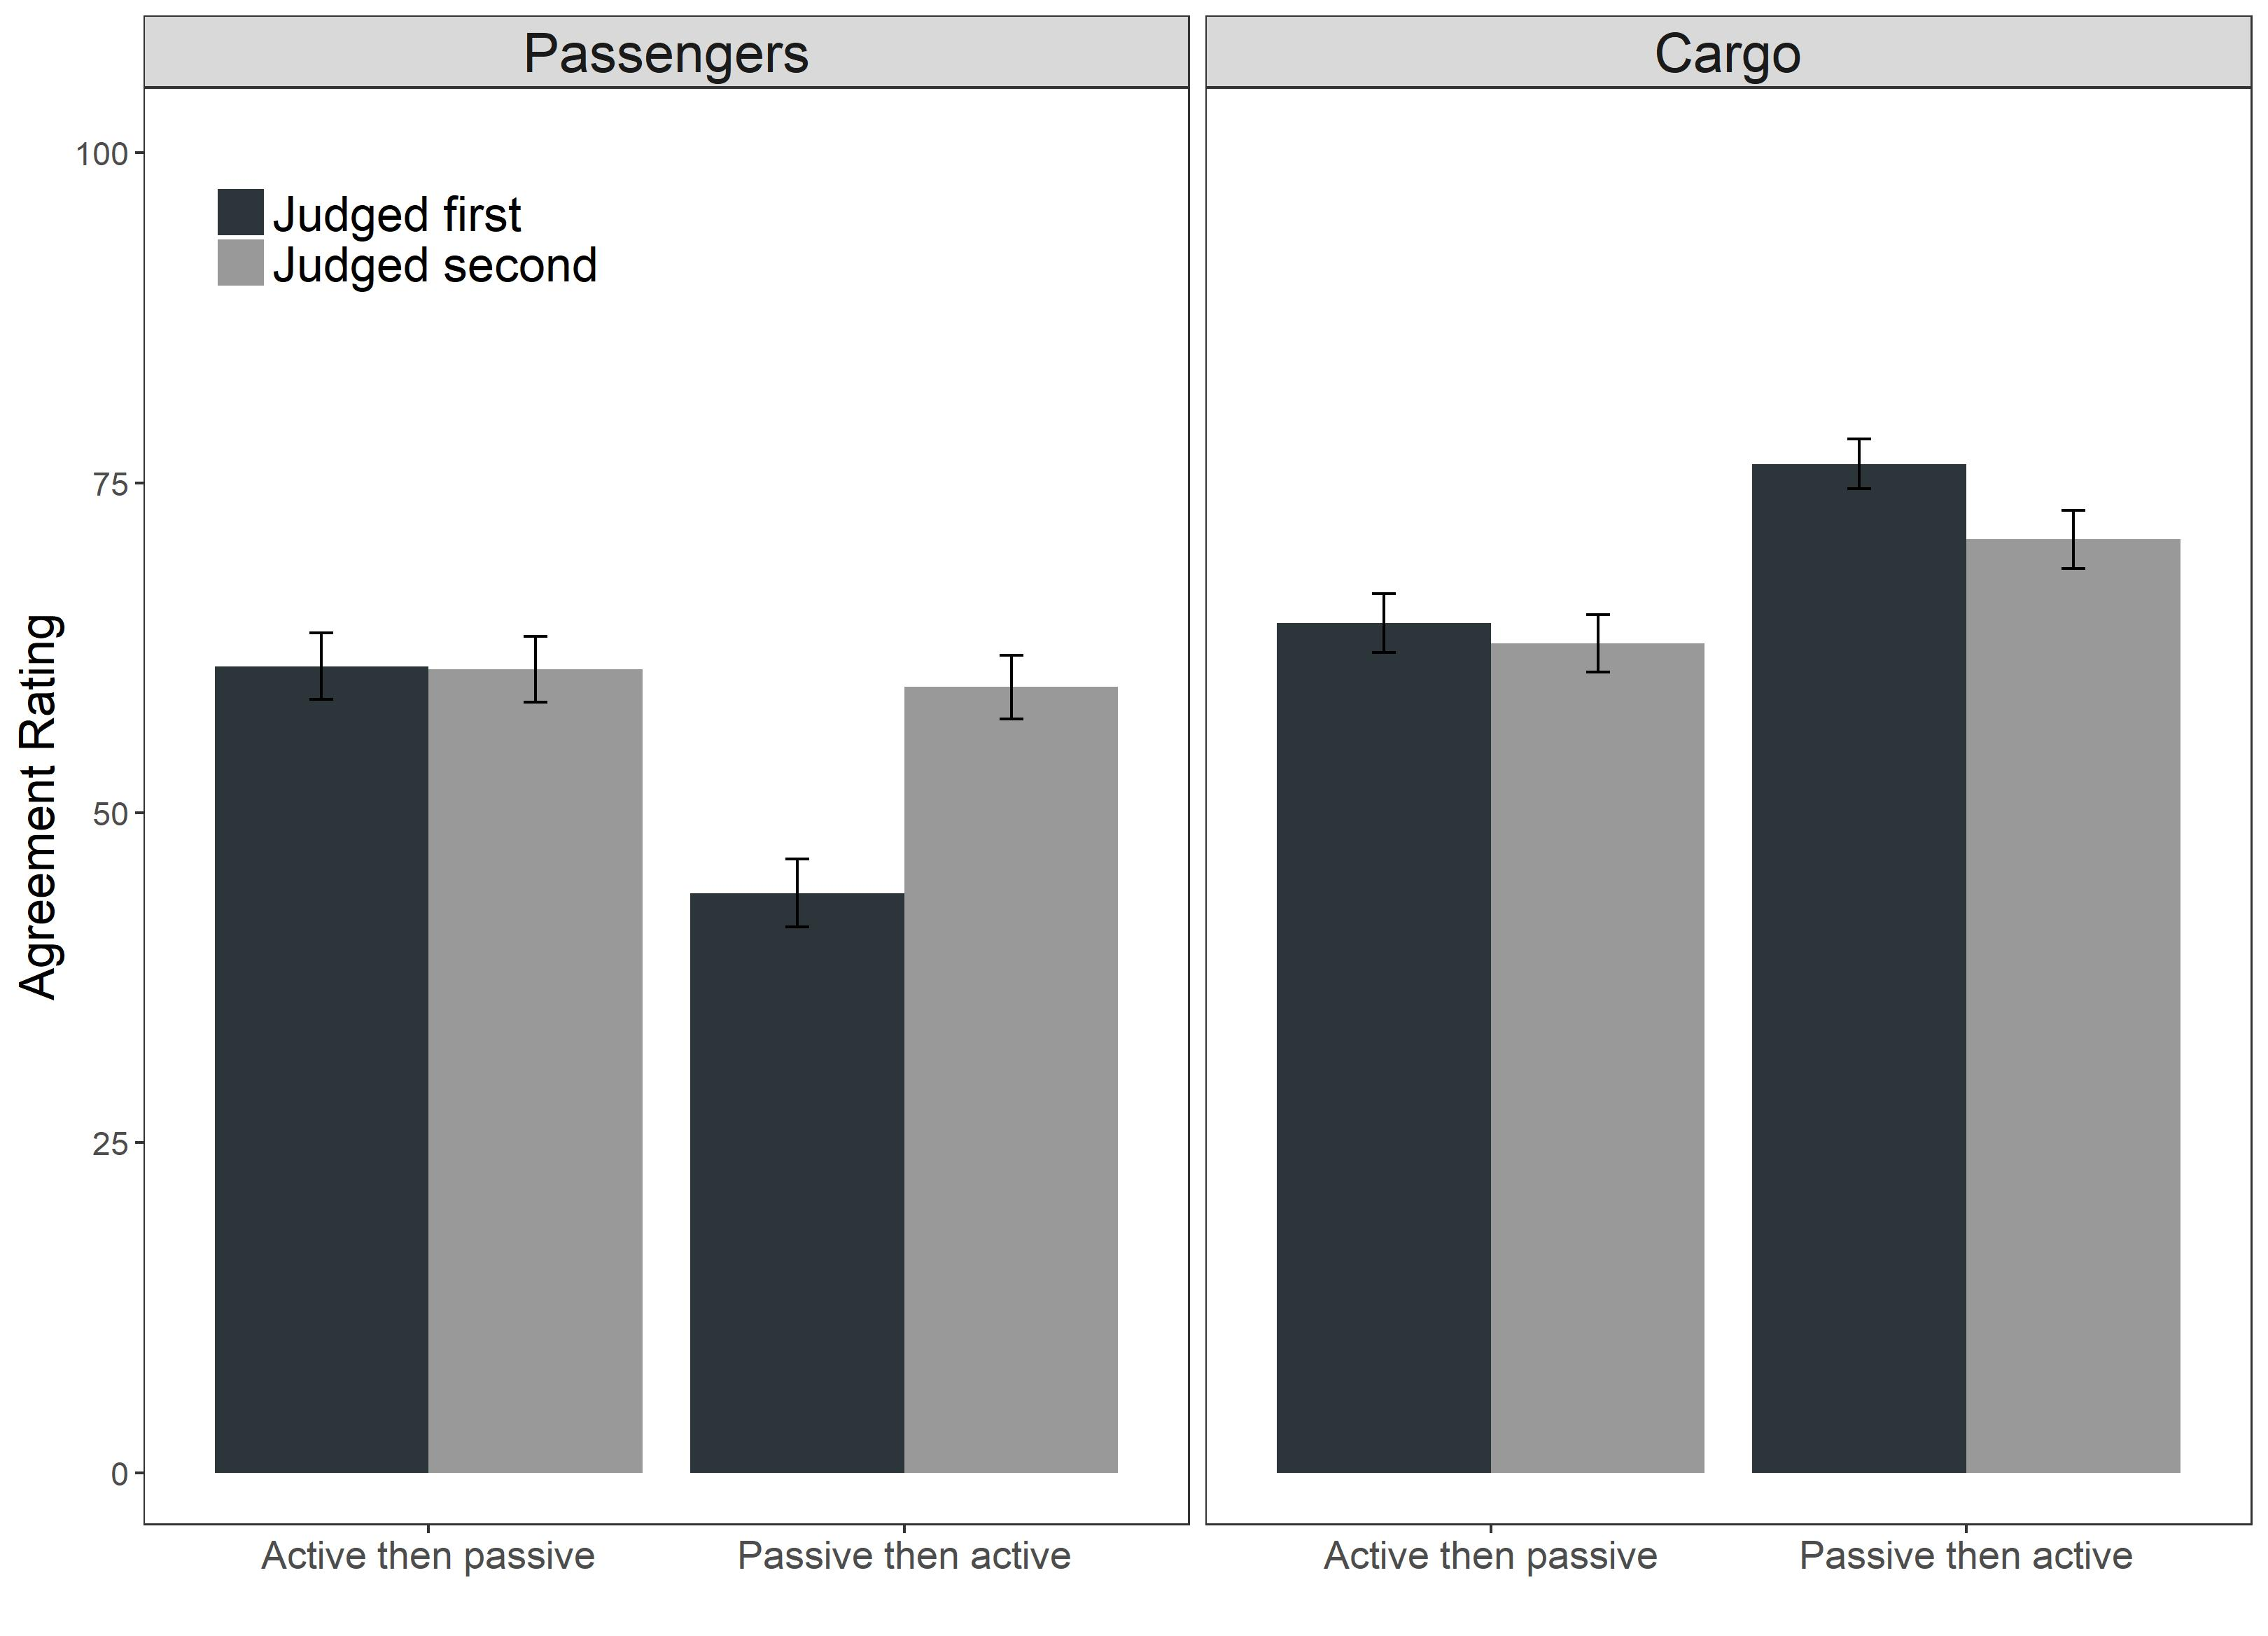
\includegraphics[width=1\linewidth]{Fig1} 
	\caption{\small Mean agreement rating with force statements when the passengers (left panel) or cargo (right panel) were thrown overboard. Within each panel, agreement with the sentence sequence in \reff{capt-sail} is on the left while agreement with the sequence in \reff{sail-capt} is on the right. Color indicates whether the sentence was judged first (dark bars) or second (light bars). Error bars indicate $+/-1$ $SEM$.}\label{Fig1}
\end{figure}

When the passengers were thrown overboard, we observed the hypothesized interaction between sentence sequence and judgment order, $\chi^2(1)=28.997$, $p<.001$. This interaction can be characterized as follows. In the sequence in \reff{sail-capt}, participants agreed less with the passive form (judged first) ($M=43.92$, $SD=36.2$) than with the active form (judged second) ($M=59.5$, $SD=34.0$), $t(395) = -4.427$, $p<.001$, $d=0.444$. In the sequence in \reff{capt-sail}, by contrast, there was no significant difference in agreement with the active form (judged first) ($M=61.1$, $SD=35.5$) and the passive form (judged second) ($M=60.9$, $SD=35.2$), $t(399) = 0.061$, $p=.952$, $d=0.006$.

When the cargo was thrown overboard, we observed a weaker interaction between sentence sequence and judgment order, $\chi^2(1)=4.093$, $p=.043$. This interaction arose from a qualitatively different pattern. In the sequence in \reff{sail-capt}, participants agreed \textit{more} with the passive form of the sentence (judged first) ($M=76.4$, $SD=26.9$) than with the active form of the sentence (judged second) ($M=70.7$, $SD=30.9$), $t(401) = 1.983$, $p=.048$, $d=0.198$. In the sequence in \reff{capt-sail}, there was again no difference in participants agreement with the the active form (judged first) ($M=64.4$, $SD=31.8$) and the passive form (judged second) ($M=62.8$, $SD=31.0$), $t(406) = 0.493$, $p=.622$, $d=0.049$.

Finally, to further characterize the observed effects, we investigated the direction of the shift in agreement with the passive sentences before vs. after reading the active sentences. In the passengers conditions, participants less agreed with the passive form of the sentence before reading the active sentence ($M=43.92$, $SD=36.2$) than after reading the active sentence ($M=60.9$, $SD=35.2$), $t(399) = -4.756$, $p<.001$, $d=0.475$. In the cargo conditions, by contrast, participants agreed with the passive sentence \textit{less} after reading the active sentence ($M=62.8$, $SD=31.0$) than before ($M=76.4$, $SD=26.9$), $t(397.15) = 4.720$, $p<.001$, $d=0.468$.

%@jonathan: what about comparing the active vs. active sentences in each  scenario? I'm wondering if there is a significant difference. obviously not in the passenger scenario. what about the cargo? if yes, as it appears, probably not worth including; but if no, that would be interesting as it would provide further evidence for quant domain. 

%% @matt: I ran that test -- basically you do find a very small effect in the cargo version: In the cargo conditions, participants agreed with the active sentence \textit{more} after reading the passive sentence ($M=70.7$, $SD=30.9$) than before ($M=64.4$, $SD=31.8$), $t(403) = 2.040$, $p=.042$, $d=0.203$. 

%% Another way to ask whether there is this efect is to ask whether you get a significant difference in agreement with the active sentences before/after reading the passive sentence \emph{across} the cargo/passengers cases. If you ask the question this way, you don't find a significant effect. If you want to include that kind of analysis instead, it'd be something like: 

% Looking across the cargo and passenger cases, we did not find that agreement with the the active form of the sentences depended on whether participants had previously judged the passive form of the sentence, $F(1,798)=1.087$, $p=.298$, $\eta^2_p=.001$.

What do these results show? Let us focus first on the passenger scenario. These results evidence exactly the kind of effect we would expect if a quantifier domain expansion hypothesis were correct. Agreement with the `force' sentences is lower when we start with the passive version, highlighting the sailor's contribution; it increases when the captain is subsequently attended to. By contrast, in the reverse, active-passive, order, agreement is relatively high when the captain is first attended to, and remains unchanged when we then attend to the sailor; in both cases it is at roughly the same point as in the active variant of the passive-active order. This evidences the ``sticky'' rates of agreement characteristic of quantifier domain expansion, with the higher agreement, active voice judgments (which focus attention on the captain) being the stickier ones---and thus the ones that go along with a larger domain of quantification. 

Intriguingly, we don't find the same pattern in the cargo scenario. Here we have mid-point agreement with both sentences in the passive-active sequence. In the active-passive order, we have elevated agreement with the active sentence, and then slightly lower, but still elevated, agreement with the passive sentence. Given the relatively small difference between these judgments, it is not exactly clear how to interpret these data. If there were a clearer contrast across the passive-active sequence, so that the active variant was closer to the midpoint and thus to both variants in the active-passive sequence, we would have clearer evidence for a quantifier domain hypothesis here---but in the opposite direction as in the passenger case. As things are, however, the evidence in the cargo scenario is unclear.

%These results not only support the quantifier domain hypothesis, but also provide two key further empirical insights. First, in our paradigm it is \emph{elevated} agreement judgments which are the sticky ones. This suggests that the quantifier domain {expansion} observed in this case goes along with \emph{elevated} agreement with `force'-claims. Second, we have evidence that it was attending to the \emph{captain} in particular which expanded the domain, since the active sentences, which focus attention on the captain, went along with the higher rates of agreement. This suggests, in turn, that we need an account of the meaning and use of `force' on which drawing attention to the captain expands some relevant domain, and this domain expansion goes along with increased agreement in `force' statements.




\section{The meaning of `force'}\label{sec:account}

%The basic idea of our account, building on \citet{Hawthorne:2001}'s contextualist proposal about `able', is that the interpretation of `force' varies with a contextual domain which represents the \emph{causal background} that we are taking into account in a given situation. The basic intuition is very close to Hawthorne's: the more causes we take into account in a situation, the more we are inclined to say that someone was unable to do otherwise than they did; and so the more willing we are to say that someone was forced to do what they did. And in our case, attending to the captain in particular makes salient this element of the situation's causal background, leading to a tendency to take it into account in assessing `force' judgments, and thus leading to the sticky increase in agreement with `force' judgments in our case. The rest of this section will be devoted to spelling out this account. 

%\subsection{`Force'}

In this section, we will take a step back from the experimental data presented so far and develop a semantics of `force' which we will then argue argue can help us make sense of those data. In particular, we propose that the following provides a plausible semantics (we formulate this in the active voice, but we assume that, at a semantic level, the active and passive formulations are equivalent):

\begin{exe}\ex \label{102}\sem{c,w}{A forced B to $\varphi$}$=1$ iff the following are true in $\seq{c,w}$: 

\begin{itemize} 
\item[(i)] `B did \sem{c}{$\varphi$}'; \item[(ii)] `B was unable to refrain from \sem{c}{$\varphi$}'; \item[(iii)] `A made (ii) true'; and \item[(iv)] `If (ii) had not been true, then B would not have done \sem{c}{$\varphi$}'.
\end{itemize}
\end{exe}

\noindent The first clause here ensures that `force' is a success term: if Sue forced John to eat a cookie, then John must indeed have eaten a cookie. The second clause encodes the sense of \emph{compulsion} characteristic of `force' judgments: if Sue forced John to eat a cookie, then John must have been \emph{compelled} to eat the cookie; there must be a sense in which John was unable to do otherwise than eat the cookie. The third clause ensures that the forcer played the right kind of role in bringing about this compulsion: it is because of Sue that John was unable to do otherwise. The role of the final clause is to rule out Frankfurt-style cases involving `force'. Suppose that Sue ensured that John could not do otherwise than eat a cookie, but John nonetheless ate a cookie completely of his own accord. In such a case, we do not want to say he was forced to eat a cookie. The fourth clause ensures that in situations like this, `force' sentences will be false.

We think this provides a plausible first-pass account of the meaning of `force', and provides a foothold in accounting for the effects of morality on judgments about force. We think that at least \emph{one} source of the sensitivity of `force' to morality and attention comes by way of the second component in the semantics here: `force' entails a lack of ability, and judgments of morality and attention can affect ability ascriptions. Consider our core scenario. In the cargo condition, we are intuitively inclined to say that the sailor \emph{could not have done otherwise than he did}; whereas in the passenger condition, we are much less inclined to say this. This suggests that morality has a similar effect on ability ascriptions as on force judgments: we are more inclined to judge agents to have been unable to do otherwise when what they do is morally neutral or good than when it is morally bad. This is exactly what we expect if `force' has roughly the meaning we suggest above and if the influence of morality on force judgments comes (at least in part) by way of the ability component of the meaning of `force'.

Moreover, the considerations Hawthorne raises provide independent intuitive evidence that attention can affect judgments about ability. Paying attention to more of the causal background of a given act can make us less likely to judge the agent as having been able to do otherwise. And in the passenger case, elevated `force' judgments corresponded with highlighting the causal background of the sailor's act---by highlighting the captain's role in the sailor's act, through Young and Phillips' active voice formulation and attention manipulation---suggesting that this may be just the mechanism that is responsible for the attention effects observed with `force'. 

We will propose, then, that judgments about `able' vary with a parameter which we will call a \emph{causal background}. The causal background is a representation which keeps track of the causal structure of a given situation. There are different ways we could spell this out formally. We will use a simple model, in which causes are true propositions (intuitively, things like the denotation of `The captain ordered the sailor to do such and such'), and the causal background is a set of propositions. In a given context, we may be happy to ignore certain features of the causal background and thereby represent agents as free to do other than they did. The more causes we take account of, however, the less we will be representing agents as free to do otherwise than they did---right up to Hawthorne's limiting case in which there is only one possibility consistent with the causal background, namely the one in which the agent does exactly as they in fact did. 

There are different ways we could integrate this kind of picture into a semantics for `able'. The simplest approach would be to build on the standard Kratzerian picture \citep{Kratzer1977,Kratzer:1981}, and simply treat `able' as a quantifier over the intersection of the causal background (or some subset thereof). But this approach has two drawbacks. One is a general concern that treating `able' as an existential quantifier over worlds in this way gives us implausibly weak truth-conditions for ability ascriptions; see \citealt{Mandelkern:2017b} for an extended recent discussion. 

A more local concern has to do with the ways in which ability ascriptions are context sensitive. In our discussion above, we noted one way in which `able' is sensitive to attention in context: drawing attention to an action's causal background can suppress agreement with ability judgments, in the way Hawthorne emphasizes. But there is another way in which ability ascriptions are context sensitive: as \citet{Mandelkern:2017b} demonstrates, drawing attention to certain \emph{actions} can \emph{increase} agreement with ability judgments. To see the point, suppose that Sue is planning to go to dinner with her friends. Ann says: 

\begin{exe}\ex Can you go to a movie tonight?\label{ann1}\end{exe}

\noindent  It's very natural for Sue to respond `No, I can't; I have dinner plans'. But now suppose that Ann replies: `So what? You \emph{could} just cancel those plans and come to the movie. So you \emph{can} go to the movie.' Once Ann has made this possibility salient, it becomes much harder for Sue to stand by her claim that she can't go. This case suggests that domain expansion in the case of ability ascriptions can go in two directions: while, as we saw above, calling attention to the \emph{causal background} of some action can durably \emph{depress} agreement with ability ascriptions, calling attention to certain  \emph{actions} available to an agent can durably \emph{elevate} agreement with ability ascriptions. And moreover, intuitively, both kinds of change are sticky in the way characteristic of quantifier domain expansion. This suggests that there are two different roles for domains of quantification in ability judgments: one domain which represents the causal background and suppresses agreement with ability ascriptions as it grows; and one which represents contextually available actions and increases agreement with ability ascriptions as it grows. 

We can capture this by building on the framework developed in \citealt{Mandelkern:2017b}. In that framework, \ul S is able to $\varphi$\ur is evaluated relative to a set of actions $\mathcal{A}$, and is true just in case there is some action $A$ in $\mathcal{A}$, such that if S tried to do $A$, she would do $\varphi$. What set of actions $\mathcal{A}$ amounts to is determined by context (Mandelkern et al. call this the set of \emph{practically available actions}); importantly, expanding that set of actions will \emph{elevate} agreement with ability ascriptions, since it will expand the possible paths for S to do $\varphi$ that we are treating as salient in a given context. This account thus nicely captures the second kind of domain-sensitivity we explored just now. To capture the first kind, we can distinguish  a separate parameter which represents the context's causal background, and which provides the building blocks for the practically available actions. More formally, let $\mathcal{C}$ denote the causal background---again, a set of propositions representing the salient causal structure of the situation in question. We can then think of $\bigcap\mathcal{C}$ as the building blocks for $\mathcal{A}$: $\mathcal{A}$ will be a set of propositions whose elements are all in $\bigcap\mathcal{C}$. Then, crucially, as $\mathcal{C}$ grows---as we take into account more of the causal background---$\mathcal{A}$ will correspondingly generally shrink, as we exclude from $\bigcap\mathcal{C}$ worlds that were in elements of $\mathcal{A}$. And so, while expanding the set of practically available actions will durably elevate agreement with ability ascriptions, expanding the causal background by attending to more of the causal structure of a given situation will durably depress agreement with ability ascriptions. 

Putting these pieces together formally: where $\wp(\bigcap\mathcal{C}_{c,w})$ is the powerset of the intersection of the causal background $\mathcal{C}_{c,w}$ at a given context $c$ and world $w$, and $f_c$ is the contextual selection function from \citet{Stalnaker68}'s theory of conditionals, which takes a proposition and a world to the ``closest'' world where that proposition is true:

\begin{exe}\ex \sem{c,w}{S is able to $\varphi$} \begin{xlist} \ex is defined only if $\mathcal{A}_{c,w}\subseteq \wp(\bigcap\mathcal{C}_{c,w})$; \ex where defined, is true iff $\exists A\in\mathcal{A}_{c,w}$ such that $f_c(\emph{S tries to do A},w)\in\sem{c,w}{S does $\varphi$}$\label{ableb} \end{xlist}\end{exe}

\noindent Informally, \ul S is able to $\varphi$\ur is true just in case there is some practically available action which entails everything in the causal background, and which is such that if S tries to do that action, she does $\varphi$.

\citet{Mandelkern:2017b} motivate the core truth conditions given in \reff{ableb}, and we won't focus on them here. What is important for present purposes is that this approach captures the dual roles of domain expansion in ability ascriptions. On the one hand, attending to more causal background, as in Hawthorne's fatalistic reverie, will expand the causal background and thus shrink the set of practically available actions. This will reduce the number of possible ways we take into account when thinking about whether the agent could bring about $\varphi$---and thus durably diminishing agreement with ability ascriptions. In the limiting case---determinism---the causal background includes every causal factor that constrained the agent's action, resulting in it being the case that the only practically available action is what the agent actually did. On the other hand, directly attending to certain actions, as in Ann's reply `So what? You \emph{could} just cancel those plans and come to the movie', can {expand} the range of actions we treat as practically available. This will increase the number of possible ways we take into account when thinking about whether the agent could bring about $\varphi$, and thereby durably increase agreement with ability ascriptions.

\section{Explaining our data}

%why difference in cargo vs. passenger order effects? in the cargo case, the captain vs. sailor formulation highlights different parts of the truth conditions of 'force'. the former highlights q. of WHO/WHAT CAUSED the sailor to be unable to do otherwise, while the sailor formulation highlights q. of whether the sailor was caused to be unable to do othrwise (by something or other). once question si raised, seems somewhat durable.  by contrast, in the passenger case, ONCE WE TAKE ON BAORD THAT THE SAILOR was unable to do otherwise, the 'cause' question is much less relevant, b/c people are much more willing to ascribe causality when something is morally bad.

With these semantics in hand for `force' and `able', let us revisit the experimental results discussed in the first part of the paper. First, to explain the basic effect of morality, we will assume that something along the lines of what Knobe and Szab\'{o} proposed is correct, appropriately generalized to the present framework. That is, we assume that subjects generally work with a causal background whose intersection includes possibilities in which people do the right thing---and thus with corresponding sets of actions which include actions which do not violate moral norms.  This means that in cases like the passenger scenario above, subjects will be less likely to take into account the full causal background which led the sailor to throw the passengers overboard, and they will be more likely to include actions in the set of practically available actions in which the sailor does something other than what he actually did, than in the cargo scenario.

But this tendency to treat agents as free to do morally good acts can run against a countervailing tendency when we call attention to more of the causal background in a given situation. In particular, highlighting the captain's causal role in bringing about the sailor's action---for instance, by using  the active voice, or highlighting the captain when describing the scenario---will tend to make us more likely to include in the causal background propositions that capture the captain's causal role: e.g., the propositions that the captain ordered the sailor to throw the passengers overboard, that the captain was a superior to the sailor, and so on. Given our semantics for `able' above, this in turn will make us less likely to treat the sailor as able to have done otherwise than he in fact did. And, given our semantics for `force', that, in turn, will make us \emph{more} likely to say that the sailor was forced to do what he did: for on our semantics for `force', `The captain forced the sailor to throw the passengers overboard' can only be true if the sailor was \emph{not} able to do otherwise than throw the passengers overboard. In short, decreasing agreement with `The sailor was able to do otherwise than throw the passengers overboard' by expanding the causal background will increase agreement with its negation, and thus tend to increase agreement with the corresponding `force'-claim.

This provides an account of the attention effects in the passenger case, and it also predicts the order effects we observed above. If quantifier domain expansion is sticky, then expanding the causal background will lead to \emph{durably} lower agreement with ability ascriptions, and thus to durably higher agreement with force ascriptions. And this is just what we observe: if we first focus attention on the sailor and then focus attention on the captain, we see an increase across the sequence in rates of agreement; whereas if we start by focusing attention on the captain and then subsequently focus on the sailor, we start from the beginning with relatively high rates of agreement in the `force'-claim, and this stays stable across the sequence.


As we saw above, we do not find similar order effects in the cargo case. A natural explanation of this is that in the cargo case, we are less likely to be ignoring the captain's causal role in the first place, and so calling attention to the captain does not change judgments in the same way. As we noted above, there is variation in the judgments in the cargo case. They seem to be consistent with quantifier domain variation, but are nowhere near as clear as the pattern in the passenger case, and go in the opposite direction. We do not see a natural way to tell a quantifier domain story about these judgments. Another possibility is that the differences in judgments observed here has to do with independent factors having to do with the questions made salient by active vs. passive formulations and the meaning of `force', but not to do with quantifier domains. More work is needed on this topic.

%Moreover, the account we have given of the semantics of `force' suggests a natural explanation of the pattern we find for sequences of `force'-claims in the cargo manipulation. Recall, again, that agreement with both statements in the active-passive condition was around the midpoint, while agreement in the passive-active condition was higher for both statements, and that this pattern did not evidence a clear pattern of quantifier domain expansion. We suspect that this pattern has to do, not with the second necessary condition on `force'-claims (which we  have focused on so far), but rather with the third requirement---that the captain \emph{made} it the case that the sailor was unable to do otherwise than he did. As we know from the basic Knobe effect, insofar as participants accept that the sailor was unable to do otherwise than he did, they will be much more likely to conclude that the \emph{captain} is the cause of this fact in the morally bad (passenger) condition than in the morally neutral (cargo) condition. In the morally neutral condition, they will be more likely to take into account other causes, like the storm. A question that asks about whether the captain forced the sailor to throw the cargo overboard naturally focuses attention on the question of whether it was the \emph{captain} who did this or something else (like the storm); whereas a question that asks whether the sailor was forced to throw the cargo overboard by the captain is more naturally heard as asking about whether the sailor was forced or not, with less emphasis on the question of whether it was the captain or something else that forced him. Thus the passive formulation of the question will be more likely to get agreement than the active, as we found (and as Young and Phillips did as well). If we assume that the question under discussion is generally durable across sequences like these, this also explains why rates of agreement are relatively stable across the sequences in both cases. The reason we don't find a similar effect in the passenger condition, again, is that, due to the Knobe effect, in the passenger case, insofar as participants accept that the sailor was unable to do otherwise than what he did, they will be more likely to conclude that the captain was the cause of this, and thus will take the third condition on `force'-claims to be satisfied uncontroversially. 


\section{Conclusion} \label{sec:conclusion}

It is now well-known that morality exerts a surprising influence on judgments about ostensibly non-moral domains such as intentionality, causality, and compulsion. In this paper we sought to make progress on understanding morality's influence by exploring subtle judgments about whether an agent was forced to do what they did. In particular, we have focused on \citet{young2011paradox}'s surprising finding that variation in whether the `force'-claims in question are formulated in the active or passive voice modulates morality's impact. We have argued that this modulation has to do with the influence of attention---which can be affected by active/passive variation, as well as by manipulating who the scenario focuses on---on a quantifier domain which affects the interpretation of `force'. We presented an experiment which showed that sequences of active versus passive `force' judgments show exactly the classic sticky pattern we expect of quantifier domain expansion. We  argued that the interpretation of `force' depends in part on a \emph{causal background} which keeps track of the causal structure of a given scenario; the more causes we take into account, the more we will judge someone to have been forced to do what they did. This provides us with the resources to make sense of the effect of  attention on `force' judgments in immoral cases.
	
In concluding, we want to step back and emphasize some of the more general upshots of our exploration. One concerns moral psychology. How should we think about the participants who show are less inclined to accept `The sailor was forced to throw the passengers overboard by the captain' than `The captain  forced the sailor to throw the passengers overboard'? One perspective, which Young and Phillips embrace, is that this inclination amounts to an `internal error', landing us amidst `logical inconsistencies'. We have suggested a different way of thinking about this inclination. On our proposal, the results in question do not point to logical inconsistencies in participants' judgments. Rather, participants in the two conditions---active vs. passive voice---are evaluating different contents, made prominent by changes in the information structure of the sentences which affect context-sensitive terms like `force', and there is nothing inconsistent about having different attitudes towards those different contents. On this alternative perspective, it would be wrong to regard the observed sensitivity to morality and attention as fundamentally erroneous. 

Of course, we might still conclude that the observed sensitivity to morality and attention is rationally suboptimal. We could try to imagine an agent whose concepts of intsentional action, causation, or compulsion were not sensitive to morality or attention. Perhaps such an agent would have one up on us rationality-wise. But perhaps not: the forms of moral context-sensitivity we have observed in natural language may turn out to be perfectly rational once one takes into account humans' fundamentally social nature and their limited capacity to represent and reason over non-actual possibilities \citep{phillips2018psychological,Phillips2017morality,Shtulman2018}. This is a central question which moral psychology must grapple with.

A second upshot is for experimental semantics and pragmatics. It is difficult to find grounds to argue that some set of judgments is a feature of context sensitivity rather than simple inconsistency or irrationality. In this paper, we have operationalized a well-known intuitive observation about quantifier domain expansion---its stickiness---showing that this feature can provide the foundations for experimental investigation of whether a given phenomenon is indeed due to changes in some domain of quantification. Specifically, the stickiness of quantifier domain expansion provides a characteristic signature in rates of agreement across sequences of the form $\seq{A,A'}$ and $\seq{A',A}$, respectively. Investigating sequences of this form should provide a solid foundation for claims about quantifier domain expansion well beyond the present inquiry. This, in turn, raises an important theoretical question which, to our knowledge, remains open, namely \emph{why} quantifier domains are sticky in this way. This question is important for understanding why the present paradigm works, and, we suspect, for better understanding the nature and sources of context-sensitivity and the cognitive effects of attention in general; it is just one of many important questions we leave open here.


\bibliography{force}   


\begin{addresses}
  \begin{address}
    Matthew Mandelkern \\
    All Souls College\\
    Oxford, OX1 4AL\\
    United Kingdom\\
    \email{matthew.mandelkern@all-souls.ox.ac.uk}
  \end{address}

  \begin{address}
   Jonathan Phillips \\
  	Harvard University\\
    1482 William James Hall \\
    33 Kirkland Street \\
    Cambridge, MA 02138\\
    USA \\
    \email{phillips01@g.harvard.edu}
  \end{address}
\end{addresses}
\end{document}



The names and addresses of all authors should be listed at the end of the
document after the bibliography, here is an example:


Brynhildur Stefánsdóttir
203 Morrill Hall
Cornell University
Ithaca, NY 14850
bs724@cornell.edu


References:

For a conference proceedings title, use the name of the society and then put
the meeting’s acronym in parentheses. Otherwise treat as a journal
article. Do not include the words “proceedings of the” or “papers from
the”.


After reviewing the suggestions above and making the changes you deem
appropriate, please upload the revised version of your paper to
http://journals.linguisticsociety.org/proceedings/index.php/SALT/, referring
to our resubmission tutorial (available in your author packet
salt28-uploading-revisions.pdf) for comprehensive instructions.
 
Thanks,
 
 
 
 
TO DO: 
-do we get an order effect asking about (i) passengers (ii) cargo; // (i) cargo; (ii) passengers; where sailor throws both overboard. different possibilities go with different theories of how the morality thing works--is it shrinking causal background, or expanding action set?

-say more about what is in causal background: basically these are categorical + conditional facts (not claims about causes, that's too circular)

-difference b/w agents and non-agents: maybe just a difference in which conditionals go into causal background (with agents, will be more responsive, fine grained)

-can we say more about how norms come into the semantics? is there a way to include them somehow in the causal background (or something)
	maybe: represent norms as generics in the CB. harder to put together generic with its counterexample (can't say 'As are phi, but some A's aren't phi' even if both are true. something similar here: we have 'People don't kill' and somehow hard to hold this together with 'X was caused to kill...')
	
-a generalization to cases of cause: A is more likely to have caused B if A had a good alternative. So the more causal background we take into account, the less people will say A caused B. Should get similar order effects. 

-redo the 'might' test with high-scope 'could'. 

-violations of non-moral norms lead to similar effects: Captain always throws Red rather than Blue. One day a storm comes up. He throws [Red/Blue]. Was he forced to throw [Red/Blue]? [Yes/no]
